\documentclass[hyperref={pdfpagelabels=false}]{beamer}

% Pacotes ----------------------------------------------------------------------
\usepackage[utf8]{inputenc}
\usepackage[T1]{fontenc}
\usepackage[brazil]{babel}

% Configurações Especializadas -------------------------------------------------
\setbeamertemplate{navigation symbols}{}
\usetheme{CambridgeUS}
\let\Tiny=\tiny

% Dados Pessoais ---------------------------------------------------------------
\title[SVN]{Subversion}
\subtitle[Versionamento]{Versionamento de Software}
\author[CAMARGO]{Wanderson Henrique Camargo Rosa}
\institute[UNISINOS]{Universidade do Vale do Rio dos Sinos --- UNISINOS}
\date{\today{}}

% Agenda -----------------------------------------------------------------------
\AtBeginSubsection[]
{
\begin{frame}{Agenda}
    \tableofcontents[currentsection,currentsubsection]
\end{frame}
}

% Início do Documento ----------------------------------------------------------
\begin{document}

% Página Inicial ---------------------------------------------------------------
\begin{frame}
    \maketitle{}
    \begin{center}
        
\includegraphics[width=20mm]{src/CC-BY-NC-SA-icon-88x31.png}
    \end{center}
\end{frame}

% Agenda -----------------------------------------------------------------------
\begin{frame}{Agenda}
    \tableofcontents{}
\end{frame}

% Introdução -------------------------------------------------------------------
\section{Introdução}
\label{sec:introducao}

\subsection{Escopo}

\begin{frame}{Escopo}
    \begin{block}{Escopo da Palestra}
        \begin{itemize}
            \item Nível
            \begin{itemize}
                \item Iniciante
            \end{itemize}
            \item Escopo
            \begin{itemize}
                \item Desenvolvimento de Software
                \item Versionamento de Software
            \end{itemize}
            \item Pré-Requisitos
            \begin{itemize}
                \item Nenhum
            \end{itemize}
        \end{itemize}
    \end{block}
\end{frame}

\subsection{Dados Pessoais}

\begin{frame}{Informações}
    \begin{block}{Dados Pessoais}
        \begin{itemize}
          \item Bacharelado em Ciência da Computação
          \item Universidade do Vale do Rio dos Sinos UNISINOS
          \item Desenvolvedor PHP Zend Framework
          \item Prefeitura Municipal de Gravataí
        \end{itemize}
    \end{block}
\end{frame}

\subsection{Objetivos}

\begin{frame}{Objetivos}
    \begin{block}{Objetivos}
        \begin{itemize}
            \item Teoria de Versionamento de Software
            \item Criação de Servidor e Utilização do Subversion
            \item Aplicação em Projetos
        \end{itemize}
    \end{block}
\end{frame}

% Teoria de Versionamento ------------------------------------------------------
\section{Teoria de Versionamento}
\label{sec:teoria}

\subsection{Controle de Versão}

\begin{frame}
    \begin{center}
        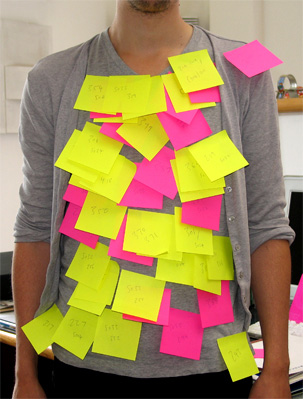
\includegraphics[width=45mm]{src/archiving72dpi.jpg}\\
        Versionamento de Software\\
        \textit{cp projeto projeto\_bkp}\\
        \textit{mv projeto\_bkp projeto\_anteontem}\\
        \textit{cp projeto projeto\_tres\_anteontem}\\
    \end{center}
\end{frame}

\begin{frame}{Teoria de Versionamento}
    \begin{block}{Controle de Versão}
        Um sistema de controle de versão é o local para armazenamento de todas
        as várias revisões de conteúdo desenvolvido enquanto criamos uma
        aplicação\cite{mason2005}. Cada revisão recebe um número que representa
        o estado do código em determinado momento. Além disso, cada revisão
        recebe uma mensagem do usuário responsável informando a causa das
        modificações.
    \end{block}
    \pause{}
    \begin{block}{Trabalho do Versionador}
        O controle de versão não somente armazena a cópia atual dos arquivos,
        mas controla as alterações já enviadas. Podemos assim, solicitar uma
        versão de arquivo específica ou efetuar uma cópia exata do documento há
        duas semanas. O servidor de controle de versões recebe o nome de
        \em{repositório}.
    \end{block}
\end{frame}

\subsection{Termos Técnicos}

\begin{frame}{Termos Técnicos}
    \begin{block}{Working Copy}
        É a cópia local de todas as informações que precisamos do repositório
        para trabalhar em nossa parte do projeto. A cópia de trabalho recebe as
        modificações do projeto, que não são salvas enquanto não são enviadas ao
        repositório. Ela recebe atualizações e modificações de outros
        colaboradores do projeto\cite{mason2005}.
    \end{block}
    \pause{}
    \begin{block}{Checkout}
        O processo de \textit{checkout} garante a criação de uma cópia de
        trabalho com as últimas revisões dos arquivos solicitados e que a
        estrutura de diretórios criada localmente será idêntica a que está no
        repositório\cite{mason2005}.
    \end{block}
\end{frame}

\begin{frame}{Termos Técnicos}
    \begin{block}{Commit}
        Envio das alterações feitas na cópia de trabalho para o repositório.
    \end{block}
    \pause{}
    \begin{block}{Update}
        Uma atualização é efetuada para solicitar as últimas revisões que estão
        no repositório. Se no servidor existirem novas atualizações de código
        que acabamos de enviar, o sistema de versionamento prioriza as suas
        alterações.
    \end{block}
\end{frame}

\begin{frame}{Estrutura Básica}
    \begin{block}{Trunk}
        A linha principal de desenvolvimento do projeto, que sempre estará em
        constante modificações\cite{mason2005}. Contém códigos ainda não
        testadose que não estão prontos.
    \end{block}
    \pause{}
    \begin{block}{Tags}
        São nomes informados para números de revisões específicas. Ao invés de
        solicitarmos a revisão \textit{r563}, podemos solicitar a revisão
        \textit{beta2}.
    \end{block}
    \pause{}
    \begin{block}{Branches}
        Linha de desenvolvimento que existe independentemente de outras linhas,
        mas que ainda compartilha uma história em comum\cite{sussman2007}.
        Sempre inicia como uma cópia de uma revisão qualquer.
    \end{block}
\end{frame}

\begin{frame}{Perguntas}
    \begin{block}{Pergunta}
        Todos os arquivos de um projeto devem ser versionados?
    \end{block}
    \pause{}
    \begin{block}{Resposta}
        \alert{Não.} Somente devem ser versionados arquivos de código-fonte.
        Arquivos que podem ser gerados a partir de outros não devem ser
        versionados.
        \begin{itemize}
            \item Imagens Temporárias (Captchas)
            \item Documentação Externa de Código (JavaDocs)
            \item Serialização de Classes em Cache (Zend Cache)
        \end{itemize}
    \end{block}
\end{frame}

\begin{frame}{Perguntas}
    \begin{block}{Pergunta}
        Cada envio de alterações pode receber um texto resumindo as modificações
        do usuário. O que deve ser escrito neste texto?
    \end{block}
    \pause{}
    \begin{block}{Resposta}
        Deve ser escrito na mensagem o porquê das modificações e não o que foi
        modificado. \alert{Exemplo:} ``Esta versão recebeu modificações de
        autenticação pois estávamos com erro de acesso ao banco de dados quando
        o usuário não digitava o seu nome''.
    \end{block}
\end{frame}

% Utilização do Versionamento --------------------------------------------------
\section{Utilização do Versionamento}
\label{sec:utilizacao}

\subsection{Criação do Servidor}

\begin{frame}{Instalação e Clientes}
    \begin{block}{Instalação}
        \begin{itemize}
            \item Ubuntu
            \begin{itemize}
                \item \$ sudo apt-get install subversion
            \end{itemize}
            \item Fedora
            \begin{itemize}
                \item \# yum install subversion
            \end{itemize}
            \item Clientes Gráficos
            \begin{itemize}
                \item Windows TortoiseSVN
                \begin{itemize}
                    \item http://tortoisesvn.tigris.org/
                \end{itemize}
                \item Eclipse Subclipse
                \begin{itemize}
                    \item http://subclipse.tigris.org/
                \end{itemize}
            \end{itemize}
        \end{itemize}
    \end{block}
\end{frame}

\begin{frame}{Servidor}
    \begin{block}{Criação do Servidor}
        \$ svnadmin create servername
    \end{block}
    \pause{}
    \begin{block}{Autenticação}
        Arquivo: servername/conf/svnserve.conf

        Linha: anon-access = read

        Linha: auth-access = write

        Linha: password-db = passwd
    \end{block}
    \pause{}
    \begin{block}{Inicialização do Serviço}
        \$ svnserve -r servername -d
    \end{block}
    \pause{}
\end{frame}

\begin{frame}{Criação do Servidor}
    \begin{block}{Acesso Cliente}
        \$ svn checkout svn://localhost/ servername
    \end{block}
    \begin{block}{Estruturação Inicial}
        \$ cd servername

        \$ svn mkdir trunk tags branches

        \$ svn commit -m ``Estrutura Inicial de Repositório''
    \end{block}
\end{frame}

\subsection{Comandos Básicos}

\begin{frame}
    \begin{block}{Adicionar Arquivos ao Versionamento}
        \$ svn add filename
    \end{block}
    \begin{block}{Enviar Modificações ao Repositório}
        \$ svn commit -m ``Mensagem para Relatório''
    \end{block}
    \begin{block}{Atualizar Modificações Recentes}
        \$ svn update
    \end{block}
    \begin{block}{Atualizar para Revisão $n$ do Repositório}
        \$ svn update -r$n$
    \end{block}
    \begin{block}{Resolver Conflitos entre Revisões}
        \$ svn resolve filename
    \end{block}
    \begin{block}{Diferença entre Modificações e Revisão Atual}
        \$ svn diff
    \end{block}
\end{frame}

\subsection{Aplicabilidades}

\begin{frame}{Aplicabilidades}
    \begin{itemize}
        \item \textit{Patches} de Software
        \item Estudo de Modificações Recentes
        \item Controle Completo do Projeto
        \item Trabalho Concorrente entre Pessoas
        \item Instalação de Módulos no Apache
        \item Utilização de Repositórios \textit{Online}
        \begin{itemize}
            \item Google Code
            \item SourceForge
        \end{itemize}
    \end{itemize}
\end{frame}

% Referências Bibliográficas ---------------------------------------------------

\begin{frame}{Referências}
    \bibliographystyle{plain}
    \bibliography{document}
\end{frame}

\begin{frame}
    \maketitle{}
\end{frame}

\end{document}